\chapter{Code and Experiments}

\section{Implementation of \FKA}

For the purpose of this thesis, we (jointly with Lacey Liang) developed a Python implementation of the \FKA{} algorithm. Using Python makes the implementation more accessible and allows for modifications that enabled a visualization of the recursion tree. We used incidence matrices to represent hypergraphs, where each row corresponds to a hyperedge and each column to a unique vertex. Existing implementations in \texttt{MATLAB} and \texttt{C}, such as \texttt{cl-jointgen} and \texttt{cl-jointgen -c}, incorporate some of the modifications we included in our implementation \cite{HKS08}.

The hypergraph dualization repository curated by Murakami and Uno \cite{Uno24} is a key resource for existing algorithms and experimental test cases related to hypergraph dualization (or solving \TransHyp). It contains several implementations in \texttt{C} and \texttt{PASCAL}. The repository also provides benchmark problem instances such as threshold graphs, uniform random hypergraphs, and hypergraphs derived from various challenging datasets.

A complete documentation of our implementation, along with explanations of the algorithm and additional tests on the primal graph properties of hypergraphs, is available in the GitHub repository: Hypergraph Transversal Thesis.

\subsection{Modifications in the Implementation of \FKA}

To ensure that the subhypergraphs in the visualization of \FKA{} recursion tree are Sperner as well, we introduced a post-decomposition Sperner reduction filter. The Sperner reduction runs the following filters:
\begin{itemize}
\item \textbf{Duplicate Removal:} The function \texttt{Unique(f, g)} eliminates duplicate edges in the hypergraph.
\item \textbf{Superset Removal:} The function \texttt{remove\_superset(np\_arr)} removes edges that are supersets of other edges. Formally, for sets $A$ and $B$, $A$ is considered a superset of $B$ if $B\subseteq A$.
\end{itemize}
These filters result in a Sperner-reduced hypergraph. Removing supersets is a practical bottleneck of the algorithm, and using optimization techniques here would speed up the algorithm's performance overall.

\paragraph{Expansion of Checking Trivial Cases:} From \ref{alg:fka}, \FKA{} tests the preconditions at each recursion level and checks whether $|G|\cdot|H|\leq 1$. If this condition is satisfied, the result is computed in $\mathcal{O}(1)$ time.

To reduce nodes on the lower recursion levels, we introduce an additional precondition to handle cases where $|G|=1$ or $|H|=1$. WLOG, if $|G|=1$, then $G$ contains a single edge $e$ such that $|e|=k$. In this case, for the input hypergraphs to be transversals, $|H|$ must equal $k$, with $H$ being a $k$-sized collection of singleton edges. This verification can be achieved in linear time, $\mathcal{O}(k)$, without necessitating further recursive calls for each vertex in $e$.

Let $G,H$ denote the input hypergraphs, and consider their decomposed subhypergraphs at depth $d$ in the recursion tree $T$, denoted $G_d$ and $H_d$. These subhypergraphs fall into one of the following categories:
\[
D_{1,k}:\ |G_d|=1,\ |H_d|=k,\quad\text{or}\quad D_{k,1}:\ |G_d|=k,\ |H_d|=1.
\]
In the naive implementation, the recursion tree $T$ will always include $D_{1,0}$, $D_{0,1}$, and $D_{1,1}$ as leaf nodes. By introducing this precondition, additional leaf nodes of type $D_{1,k}$ and $D_{k,1}$ are created, where $k\geq 2$. For each such node, the naive implementation would have required up to $k-1$ additional recursive steps to reduce to $D_{1,1}$. Our optimization eliminates these steps, significantly simplifying $T$ and reducing redundant computations.

\subsection{Visualization of the\FKA{} Algorithm and Recursion Tree}

The visualizer for the\FKA{} algorithm provides a dynamic view of its recursive structure, showcasing the evolution of hypergraphs $G$ and $H$ through transformations, splitting vertices, and recursion paths. It generates a recursion tree $T$, capturing key decisions and decompositions at each step.

The recursion tree $T$ illustrates the decomposition process:
\begin{itemize}
\item \textbf{Left Branch (L)}: Represents $(G_1,H_0\vee H_1)$.
\item \textbf{Right Branch (R)}: Represents $(H_1,G_0\vee G_1)$.
\item \textbf{Node Depth}: Each node $v$ has depth $d_v(T)$, defined as the length of the path from the root to $v$.
\end{itemize}

The splitting variable $v$ partitions $G$ and $H$ into subhypergraphs $G_0,G_1,H_0$, and $H_1$. They form the input for recursive calls, with changes annotated by the \texttt{@Visualiser} decorator

The visualizer records the frequent vertex $v$ at each step and shows the non-Sperner edges filtered out on each node. Node-specific exploration is supported via \texttt{display(node\_num)}, which outputs the intermediary hypergraphs, deleted rows, and splitting variables.

\section{Experiments and Results}

Datasets featuring hypergraphs with large transversal hypergraphs compiled in \cite{Uno24} are commonly used in the study of \FKA{} and related algorithms for solving \TransHyp{} \cite{Tak08}. This thesis looks into the symmetric properties of hypergraphs and the impact of recursion trees in \FKA. It also focuses on identifying hypergraph classes where \FKA{} faces challenges and analyze their symmetry and combinatorial properties. Thus, large recursion trees by themselves do not provide new insights for our analysis.

We used selected hypergraphs as input for \FKA{} and published their recursion trees and automorphism group trees. The hypergraph property we examined was \emph{conformality.} Conformality preserves the structure of the primal graph through their maximal cliques but does not preserve the edge-incidence structure. It is an important property for studying acyclicity in hypergraphs.

We also studied the primal graphs of these hypergraphs. We checked if they belong to specific graph classes: cographs, chordal graphs, or chordal bipartite graphs. These graph classes are subclasses of distance-hereditary graphs, and thus contain equivalence classes of twin vertices.

\subsection{Problem Instances}

We selected some familiar read-once hypergraphs $(f_2,g_2)$, and some new some new hypergraphs on small number of vertices.

Hypergraph $f_2$ and its transversal hypergraph $g_2$:
\begin{gather*}
f_2=\{\{v_1,v_3\},\{v_1,v_4\},\{v_2,v_3\},\{v_2,v_4\},\{v_5,v_7\},\{v_5,v_8\},\{v_6,v_7\},\{v_6,v_8\}\}\\[4pt]
g_2=\{\{v_1,v_2,v_7,v_8\},\{v_3,v_4,v_5,v_6\},\{v_1,v_2,v_5,v_6\},\{v_3,v_4,v_7,v_8\}\}
\end{gather*}

Hertel also presented another family of read-once hypergraphs and called it \emph{Mark's class.} It consists of Sperner hypergraphs of the form:
\[
H_q^p=c_1\wedge c_2\wedge\dots\wedge c_p
\]
where each $c_i$ in $H_q^p$ is disjoint from every other $c_j$, and $c_i$s have the form:
\[
c_i=((v_1\wedge v_2\wedge\dots\wedge v_q)\vee(v_{q+1}\wedge v_{q+2}\wedge\dots\wedge v_{2q})).
\]

Mark's class produces some hypergraphs not present in alternating trees and allows generation of both the $\GK$-family and $\TK$-family, offering a broader class of recursively generated hypergraphs. However, in our experiments, we did not observe any new characteristics that Mark's class presented and wasn't present in the alternating trees.

Recent work \cite{SS24} has employed reinforcement learning techniques to explore simple hypergraphs that have characteristics that challenge \FKA. This work highlights several natural optimization questions to frame their search of pairs of transversal hypergraphs, such as minimizing $\epsilon(G,H)$, minimizing $\log(|G|+|H|)\cdot\epsilon(G,H)$, and identifying hypergraphs that maximize the recursion tree depth for \FKA. For our experiment, we selected results that minimize $\epsilon(G,H)$ to better understand and challenge the performance of \FKA.

We only took hypergraphs on 6 vertices or larger. For notation, we are calling the hypergraphs and their transversals on 6 vertices as 6-A, 6-B, 6-C, 6-D, the hypergraph on 7 vertices and it's transversal as 7-ver and the hypergraph on 8-vertices and it's transversal as 8-ver.

\begin{itemize}
\item Hypergraph 6-A:
\begin{gather*}
G=\{\{v_1,v_5,v_6\},\{v_4,v_5\},\{v_1,v_2\},\{v_2,v_3,v_4\}\},\\[4pt]
H=\{\{v_2,v_4,v_6\},\{v_2,v_5\},\{v_1,v_4\},\{v_1,v_3,v_5\}\}
\end{gather*}
\item Hypergraph 6-B:
\begin{gather*}
G=\{\{v_1,v_3,v_5\},\{v_1,v_2,v_6\},\{v_1,v_2,v_3\},\{v_1,v_5,v_6\},\{v_3,v_4,v_5\},\\[4pt]
\{v_2,v_3,v_4\},\{v_4,v_5,v_6\},\{v_2,v_4,v_6\}\},\\[4pt]
H=\{\{v_2,v_5\},\{v_1,v_4\},\{v_3,v_6\}\}
\end{gather*}
\item Hypergraph 6-C:
\begin{gather*}
G=\{\{v_3,v_4\},\{v_1,v_5\},\{v_2,v_3\},\{v_4,v_5\},\{v_5,v_6\},\{v_3,v_6\},\\[4pt]
\{v_2,v_5\},\{v_1,v_3\}\},\\[4pt]
H=\{\{v_3,v_5\},\{v_1,v_2,v_4,v_6\}\}
\end{gather*}
\item Hypergraph 6-D:
\begin{gather*}
G=\{\{v_1,v_2,v_6\},\{v_2,v_4\},\{v_3,v_4,v_5\},\{v_1,v_3,v_5,v_6\}\},\\[4pt]
H=\{\{v_2,v_3\},\{v_2,v_5\},\{v_1,v_4\},\{v_4,v_6\}\}
\end{gather*}
\item Hypergraph 7-Ver:
\begin{gather*}
G=\{\{v_1,v_2,v_6\},\{v_1,v_5,v_7\},\{v_3,v_4,v_7\},\{v_2,v_5,v_7\},\{v_1,v_5,v_6\},\\[4pt]
\{v_1,v_3,v_7\},\{v_3,v_4,v_5\},\{v_2,v_3,v_4\},\{v_2,v_4,v_6\},\{v_1,v_6,v_7\},\{v_2,v_5,v_6\}\},\\[4pt]
H=\{\{v_3,v_6,v_7\},\{v_3,v_5,v_6\},\{v_1,v_2,v_3\},\{v_2,v_5,v_7\},\{v_4,v_6,v_7\},\\[4pt]
\{v_1,v_4,v_5\},\{v_1,v_2,v_4\}\}
\end{gather*}
\item Hypergraph 8-Ver:
\begin{gather*}
G=\{\{v_2,v_6,v_7,v_8\},\{v_3,v_7,v_8\},\{v_1,v_4,v_5\},\{v_2,v_5,v_6\},\{v_1,v_3,v_4\}\},\\[4pt]
H=\{\{v_1,v_2,v_3\},\{v_2,v_3,v_4\},\{v_2,v_3,v_5\},\{v_1,v_3,v_6\},\{v_3,v_4,v_6\},\{v_3,v_5,v_6\},\{v_1,v_2,v_7\},\\[4pt]
\{v_2,v_4,v_7\},\{v_1,v_5,v_7\},\{v_3,v_5,v_7\},\{v_4,v_5,v_7\},\{v_1,v_6,v_7\},\{v_4,v_6,v_7\},\{v_1,v_2,v_8\},\\[4pt]
\{v_2,v_4,v_8\},\{v_1,v_5,v_8\},\{v_3,v_5,v_8\},\{v_4,v_5,v_8\},\{v_1,v_6,v_8\},\{v_4,v_6,v_8\}\}
\end{gather*}
\end{itemize}

Each pair is a transversal pair (\leanref{sixA_dual}, \dots, \leanref{eightVer_dual}). The 2024 edition printed the 6-A edge $\{v_4,v_5\}$ as $\{v_4,v_5,v_6\}$ and the 8-Ver transversal with 19 edges; as printed, neither is a transversal pair (\leanref{sixA_printed_not_dual}, \leanref{eightVer_printed_not_dual}).

The Fano plane hypergraphs are an interesting case, and their family of hypergraphs have been widely used in recent literature \cite{Uno24}, defined as the following:

\begin{definition}[Self-Dual Fano-Plane Hypergraph (SDFP)]
Let $H=(V,E)$ be a hypergraph with $v$ vertices and $k=\frac{v-2}{7}$. The edge set $E_0$ of the base hypergraph corresponds to the lines in the Fano plane:
\[
H_0=\{\{v_1,v_2,v_4\},\{v_2,v_3,v_5\},\{v_3,v_4,v_6\},\{v_4,v_5,v_7\},\{v_1,v_5,v_6\},\{v_2,v_6,v_7\},\{v_1,v_3,v_7\}\}
\]
The full edge set $E$ is constructed by taking $k$ disjoint copies of $H_0$, such that $E=\bigcup_{i=1}^{k}E_i$, where each $E_i$ is a copy of $E_0$.
\end{definition}

The $k$ disjoint copies have $7k$ edges and their transversal has $7^k$ edges (\leanref{kFano_card}, \leanref{tr_kFano_card}); the 2024 edition printed $\frac{(k-2)^2}{4}+k/2+1$, which already fails at $k=2$, where the count is $49$ \leanref{two_fano_tr_card}. We are showing $H_0$ or the self-transversal fano plane hypergraph in our visualizations, refer to \cite{Uno24} for the larger constructions.

We were also interested in examining how symmetry could emerge in inherently asymmetric hypergraphs through the decomposition process and whether there are properties that could provide deeper insight into their latent symmetry and its relationship with \FKA. To this end, we constructed several 4-uniform hypergraphs on 8 vertices, each with a trivial automorphism group. We presented the results of two such hypergraphs, denoted $\mathrm{Asym}-1$ and $\mathrm{Asym}-2$.

\subsection{Results and Observations}

For the given hypergraphs, each node in the automorphism tree corresponds to a respective node in the \FKA{} recursion tree and reflects the properties of the input hypergraphs at that stage of recursion.
\begin{itemize}
\item For each node in the \FKA{} recursion tree, the input hypergraphs $G$ and $H$ (if they are transversals of each other) have the same automorphism group. If one hypergraph between $G$ or $H$ was conformal while the other was not, we noted this in the automorphism tree. Regarding primal graph properties, when the primal graphs of $G$ and $H$ exhibited differing characteristics, we highlighted the property that contributed to either a classification or a recurring structural feature, preferring recurring over non-recurring properties.
\item For read-once hypergraphs, the read-once property remained preserved throughout the recursion tree. Consequently, their hypergraph properties did not require updates at each node of the automorphism tree.
\item If no significant or distinguishing property was identified for a particular node, the corresponding entry in the automorphism tree was left empty.
\item The asymmetric hypergraphs and the Fano plane hypergraph were non-conformal. However, due to the decomposition of small cases, a few recursive steps often reduced the hypergraph sufficiently for familiar structures to emerge, exhibiting properties like read-once or acyclicity.
\end{itemize}

\subsubsection*{Read-Once Hypergraphs in \FKA}

The input hypergraphs maintained both their conformality and their read-once property throughout the decomposition process. While this relationship is not preserved in every recursive step, an interesting pattern emerges: if an input hypergraph $f$ at a given node in the automorphism tree is $\alpha$-acyclic, the primal graph of its transversal is often chordal bipartite. This suggests a potential connection between chordal bipartite graphs and hypergraph acyclicity, warranting further exploration. In our experiments, we did not observe any new characteristics that Mark's class presented and wasn't present in the alternating trees.

In the recursion tree for \FKA{} on $f_2,g_2$, we observe the following occurring:

\begin{observation}[\leanref{falseTwin_filtered}, \leanref{f2g2_false_twin_filtered}]\label{obs:false-twins}
In the \FKA{} decomposition of certain read-once hypergraphs, when the most frequent vertex is deleted, its false twin vertices are filtered out by the Sperner condition in the contraction subhypergraph. In general: if $u\ne x$ and every edge through $u$ is a pair $\{u,w\}$ with $\{x,w\}$ also an edge, then $u$ lies in no edge of $min(G/x)$.
\end{observation}

In the \FKA{} decomposition, we use $f_2,g_2$ to illustrate the observation (see Figure \ref{fig:f2g2}).

\begin{figure}[p]
\centering
\begin{subfigure}{\linewidth}\centering
\resizebox{0.95\linewidth}{!}{\begin{forest}
autotree
[{\anode{1}{$v_{1}$}{$(((C_2\times C_2\times C_2\times C_2):C_2):C_2):C_2$}{Read-Once Hypergraph}{}}
  [{\anode{2}{$v_{2}$}{$C_2\times D_4$}{}{Chordal Bipartite}}
    [{\anode{3}{$v_{5}$}{$D_4$}{}{$C_4$ graph}}
      [{\anode{4}{$v_{6}$}{$C_2$}{}{Bipartite}}
        [{\anode{5}{}{$\{\}$}{}{}}]
        [{\anode{6}{}{$C_2$}{}{}}]
      ]
      [{\anode{7}{}{$C_2$}{}{}}]
    ]
    [{\anode{8}{$v_{3}$}{$C_2\times D_4$}{$\alpha$-acyclic}{}}
      [{\anode{9}{}{$\{\}$}{}{}}]
      [{\anode{10}{$v_{4}$}{$D_4$}{}{$C_4+K_1$ graph, Chordal Bipartite}}
        [{\anode{11}{$v_{5}$}{$D_4$}{}{$C_4$ graph}}
          [{\anode{12}{$v_{6}$}{$C_2$}{}{Bipartite}}
            [{\anode{13}{}{$\{\}$}{}{}}]
            [{\anode{14}{}{$C_2$}{}{}}]
          ]
          [{\anode{15}{}{$C_2$}{}{}}]
        ]
        [{\anode{16}{}{$\{\}$}{}{}}]
      ]
    ]
  ]
  [{\anode{17}{$v_{3}$}{$C_2\times D_4$}{$\alpha$-acyclic, Read-Once}{}}
    [{\anode{18}{}{$\{\}$}{}{}}]
    [{\anode{19}{$v_{4}$}{$D_4$}{}{$C_4+K_1$ graph}}
      [{\anode{20}{$v_{5}$}{$D_4$}{}{$C_4$ graph}}
        [{\anode{21}{$v_{6}$}{$C_2$}{}{}}
          [{\anode{22}{}{$\{\}$}{}{}}]
          [{\anode{23}{}{$C_2$}{}{}}]
        ]
        [{\anode{24}{}{$C_2$}{}{}}]
      ]
      [{\anode{25}{}{$\{\}$}{}{}}]
    ]
  ]
]
\end{forest}
}
\caption{Automorphism Tree of $f_2,g_2$ from $\GK$-family in \FKA}
\end{subfigure}\\[6pt]
\begin{subfigure}{\linewidth}\centering
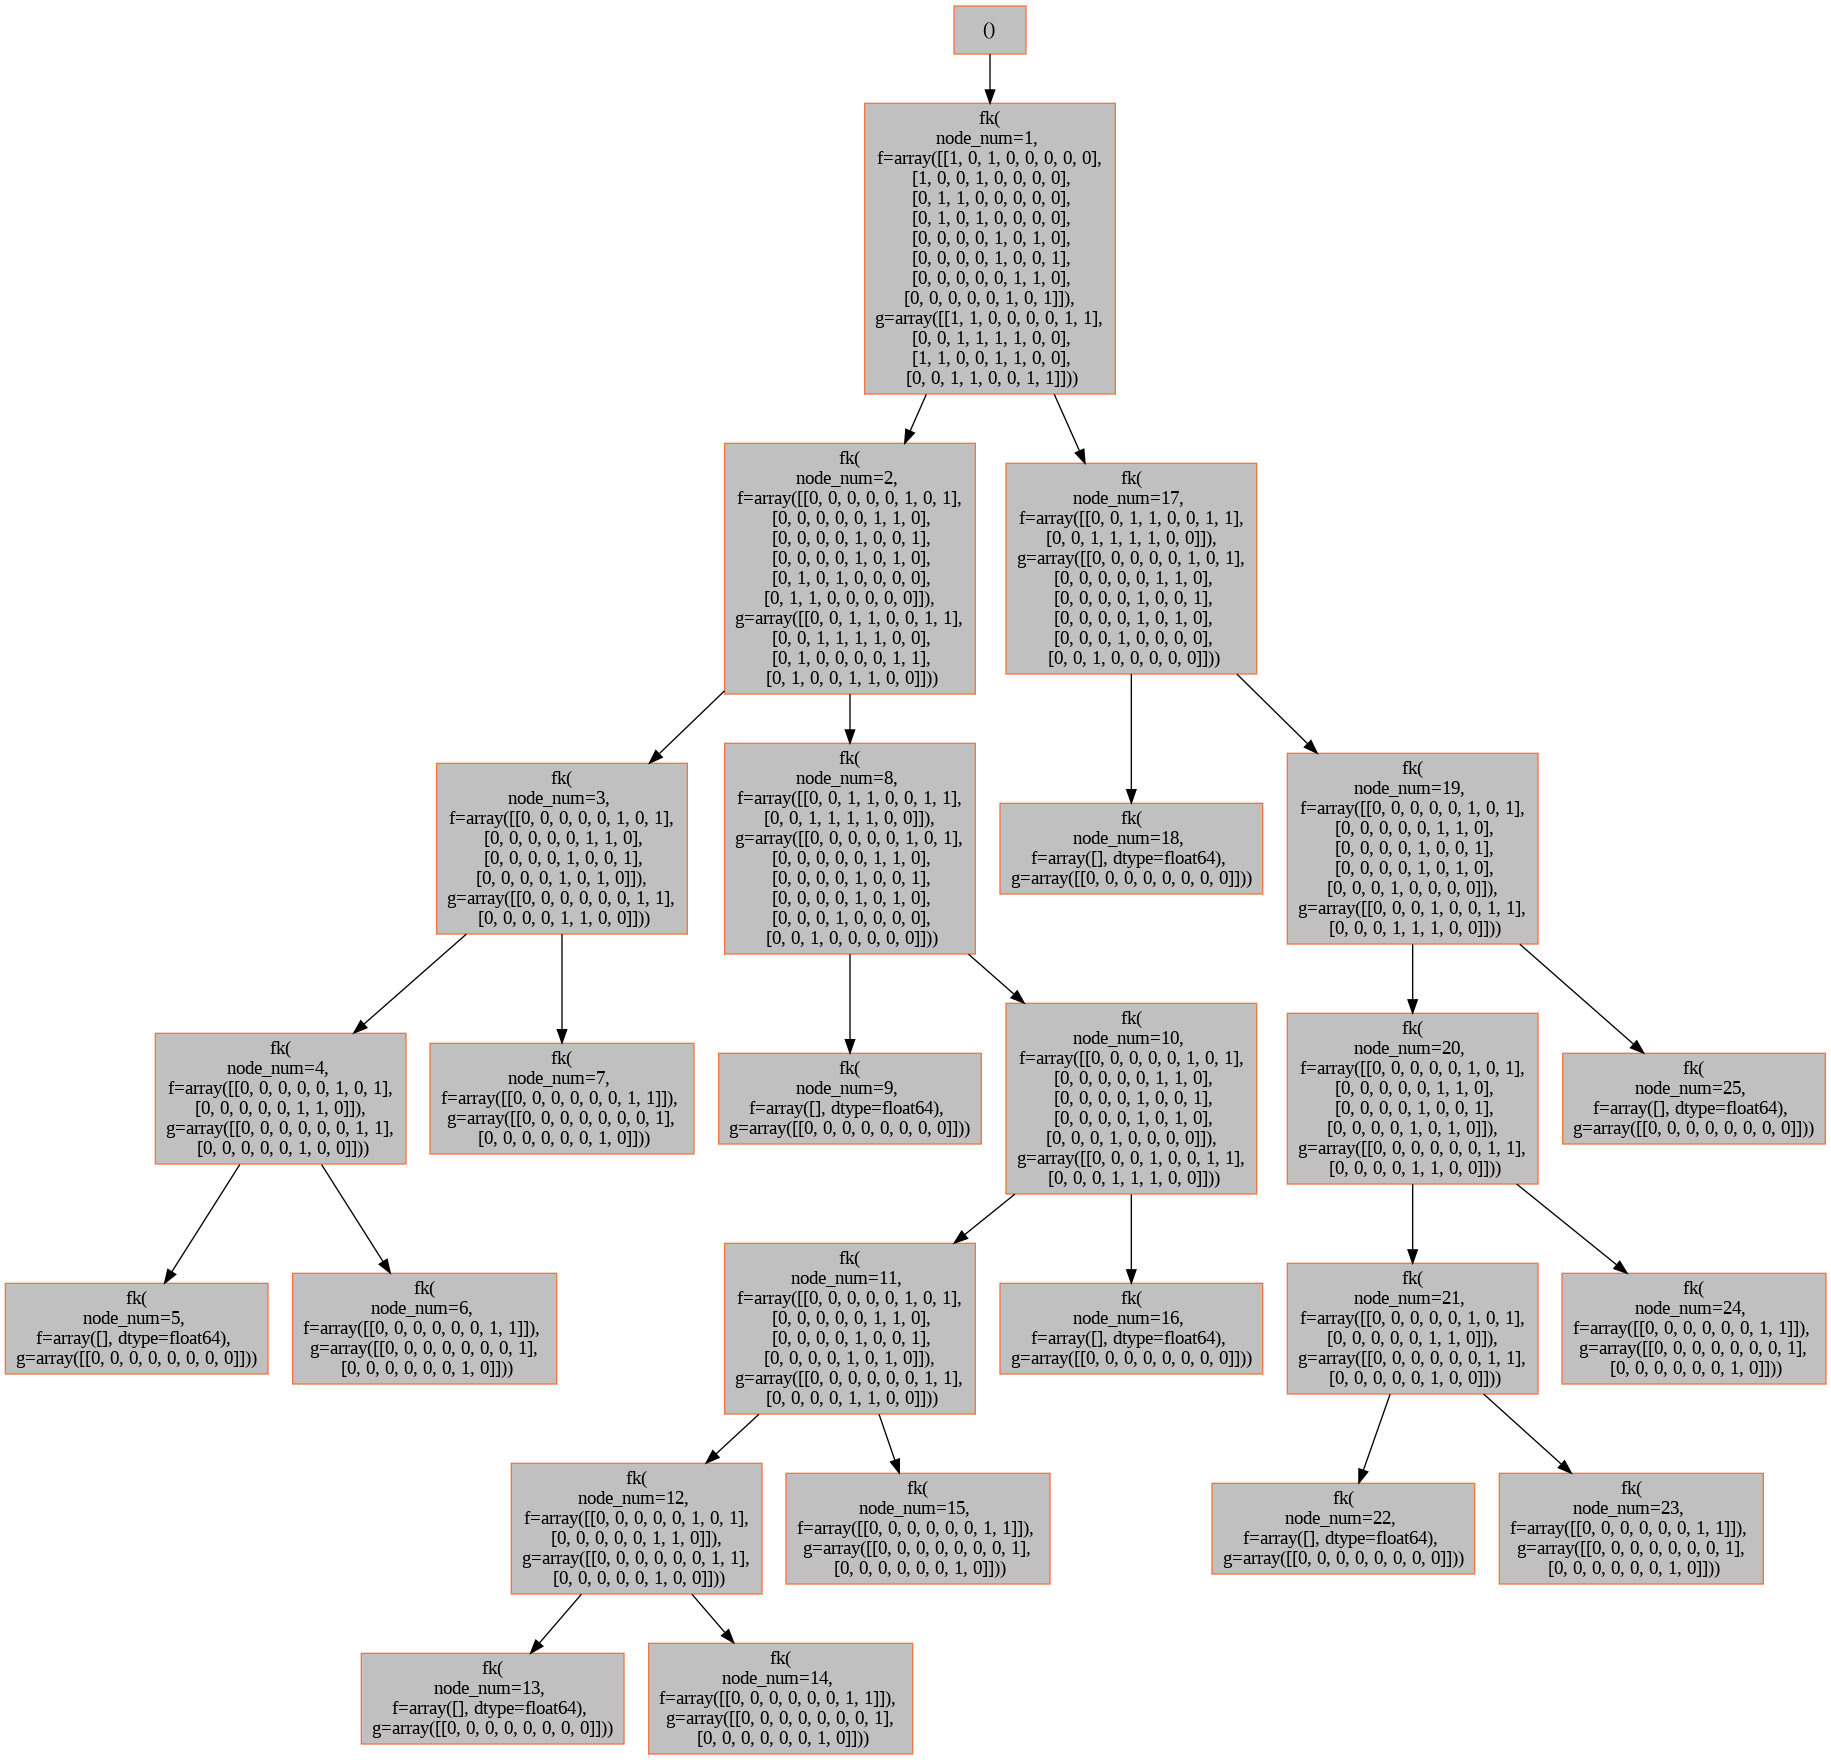
\includegraphics[width=0.62\linewidth]{figures/f2g2-fka.png}
\caption{Figures/f2, g2 in\FKA.png}
\end{subfigure}
\caption{\FKA{} recursion tree and automorphism tree of $f_2,g_2$}\label{fig:f2g2}
\end{figure}

We note that the twin classes are creating a direct product that's acting as a normal subgroup and the base group of the wreath product, supporting \ref{prop:cameron}. At Node 1, for $f_2$, the most frequent vertex is $v_1$, whose false twin partner is $v_2$. When $v_1$ is deleted and the \emph{contraction} subhypergraph $f_0\vee f_1$ is formed at Node 19 (denoted as $g$), we observe that two vertices are lost from the hypergraph. However, this is not explicitly shown in \FKA, as isolated vertices are not permitted, whereas singleton edges (edges containing a single vertex) are included.

In the corresponding \emph{deletion} subhypergraph at Node 2, we observe that no additional vertices disappear. At Node 19, the remaining two singleton edges are part of both hyperedges in their transversal. Selecting either of these singleton vertices as the next pivot vertex prunes the \textbf{L} subproblem at Node 18.

Furthermore, at Node 2, $v_2$ is selected as the most frequent vertex. The resulting contraction subhypergraph at Node 8 is identical to that at Node 17. This repetition of subproblems contributes to the enlargement of the recursion tree in \FKA.

The hypergraphs who are both read-once and $\alpha$-acyclic, have an interesting property in their primal graphs. Since cographs are distance-hereditary and they are also chordal (\ref{def:chordal}), these primal graphs are precisely the class of Ptolemaic graphs. We haven't found a classification for the families of hypergraphs when their primal graphs are chordal bipartite, or Ptolemaic in existing literature or their impact on the performance of the \FKA{} algorithm.

As we have previously discussed, Cameron proposed \cite{Cam22} that the automorphism group of cographs can be generated by taking direct products and wreath products with a symmetric group. Now, we get to see if that holds up for the corresponding clique hypergraphs.

Let's consider $G$, the disjoint union of 2 disjoint $C_4$, denoted $G_1,G_2$. The automorphism group $\Aut(G)$ must preserve the twin structure of each $C_4$ while allowing permutations between the two disjoint cycles.

We describe the structure of $\Aut(G)$ as follows:
\begin{itemize}
\item The base group $C_2\times C_2\times C_2\times C_2$ corresponds to independent actions on the twin classes $\{v_1,v_3\}$, $\{v_2,v_4\}$, $\{v_5,v_7\}$, and $\{v_6,v_8\}$.
\item The first top group $C_2$ permutes the twin classes within each connected structure independently.
\item The second top group $C_2$ permutes the two disjoint components $G_1$ and $G_2$.
\end{itemize}

Combining these, $\Aut(G)$ is isomorphic to the iterated wreath product:
\[
\Aut(G)\cong(((C_2\times C_2\times C_2\times C_2):C_2):C_2):C_2.
\]
This reflects the hierarchical structure of symmetries in $G$. This is also isomorphic to $D_4\wr S_2$, where the outer $S_2$ permutes the disjoint cycles.

Therefore, we see that our results support Cameron's proposition (\ref{prop:cameron})on the primal graph of read-once hypergraphs.

\subsubsection*{Fano Plane Hypergraph}

\begin{figure}[p]
\centering
\begin{subfigure}{\linewidth}\centering
\resizebox{\linewidth}{!}{\begin{forest}
autotree
[{\anode{1}{$v_{1}$}{$PSL(3,2)$}{Not Conformal}{Cograph, Chordal}}
  [{\anode{2}{$v_{2}$}{$S_4\text{ (Non-terminal)}$}{Not Conformal}{Cograph, Split, Chordal}}
    [{\anode{3}{$v_{3}$}{$D_8$}{$\alpha$-acyclic, ROH}{}}
      [{\anode{4}{}{$S_3$}{}{}}]
      [{\anode{5}{$v_{4}$}{$C_2$}{$\alpha$-acyclic, ROH}{}}
        [{\anode{6}{$v_{6}$}{$C_2$}{}{}}
          [{\anode{7}{}{$\{\}$}{}{}}]
          [{\anode{8}{}{$C_2$}{}{}}]
        ]
        [{\anode{9}{}{$\{\}$}{}{}}]
      ]
    ]
    [{\anode{10}{$v_{3}$}{$C_2\times C_2$}{}{Cograph}}
      [{\anode{11}{$v_{5}$}{$C_2$}{$\alpha$-acyclic, ROH}{}}
        [{\anode{12}{}{$\{\}$}{}{}}]
        [{\anode{13}{$v_{6}$}{$C_2$}{}{}}
          [{\anode{14}{}{$\{\}$}{}{}}]
          [{\anode{15}{}{$C_2$}{}{}}]
        ]
      ]
      [{\anode{16}{$v_{6}$}{$C_2$}{$\alpha$-acyclic, ROH}{}}
        [{\anode{17}{}{$S_3$}{}{}}]
        [{\anode{18}{}{$S_1$}{}{}}]
      ]
    ]
  ]
  [{\anode{19}{$v_{2}$}{$S_4\text{ (Non-terminal)}$}{Not Conformal}{Cograph, Split, Chordal}}
    [{\anode{20}{$v_{3}$}{$D_4$}{$\alpha$-acyclic, ROH}{}}
      [{\anode{21}{}{$S_3$}{}{}}]
      [{\anode{22}{$v_{4}$}{$C_2$}{$\alpha$-acyclic, ROH}{Split}}
        [{\anode{23}{$v_{6}$}{$C_2$}{}{}}
          [{\anode{24}{}{$\{\}$}{}{}}]
          [{\anode{25}{}{$C_2$}{}{}}]
        ]
        [{\anode{26}{}{$\{\}$}{}{}}]
      ]
    ]
    [{\anode{27}{$v_{3}$}{$C_2\times C_2$}{}{Cograph}}
      [{\anode{28}{$v_{5}$}{$C_2$}{$\alpha$-acyclic, ROH}{Split}}
        [{\anode{29}{}{$\{\}$}{}{}}]
        [{\anode{30}{$v_{6}$}{$C_2$}{}{}}
          [{\anode{31}{}{$\{\}$}{}{}}]
          [{\anode{32}{}{$C_2$}{}{}}]
        ]
      ]
      [{\anode{33}{$v_{6}$}{$C_2$}{$\alpha$-acyclic, ROH}{Split}}
        [{\anode{34}{}{$S_3$}{}{}}]
        [{\anode{35}{}{$C_1$}{}{}}]
      ]
    ]
  ]
]
\end{forest}
}
\caption{Automorphism Tree of Self-Transversal Fano Plane Hypergraph in \FKA}
\end{subfigure}\\[6pt]
\begin{subfigure}{\linewidth}\centering
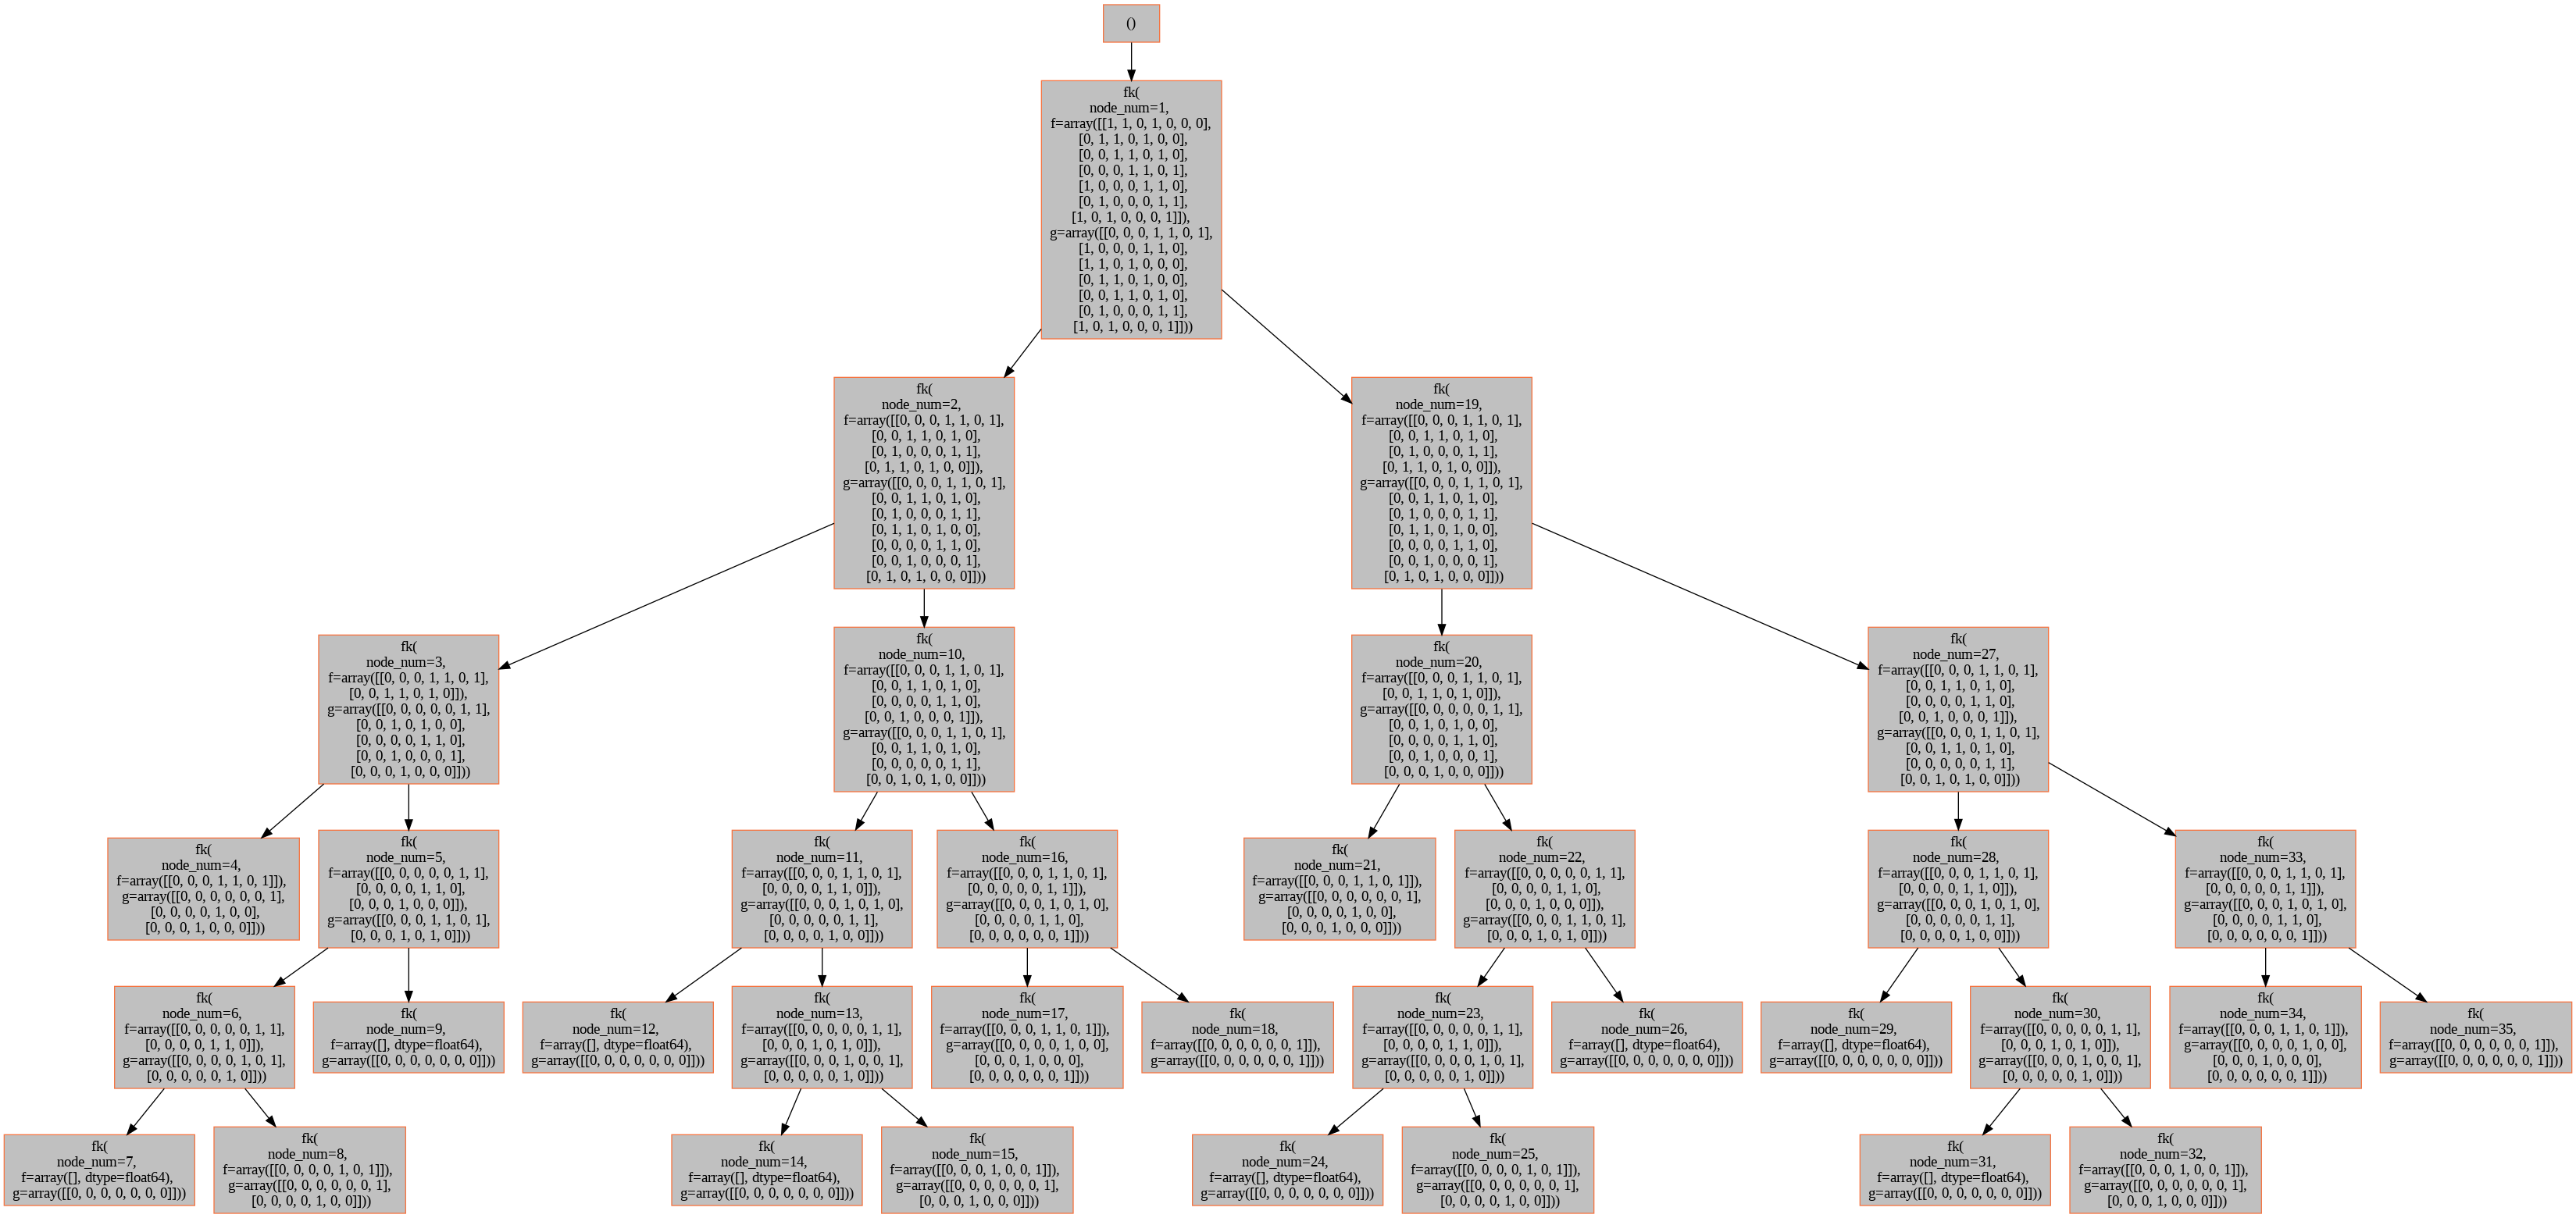
\includegraphics[width=0.8\linewidth]{figures/fano-fka.png}
\caption{Fano Plane Hypergraph in \FKA}
\end{subfigure}
\caption{\FKA{} recursion tree and automorphism tree of the Fano Plane}\label{fig:fano}
\end{figure}

Before discussing the hypergraphs from \cite{SS24}, we note the following:

\begin{observation}[\leanref{eps_three}, \leanref{eps_four}, \leanref{eps_seven}, \leanref{fano_eps}]\label{obs:fano-tight}
Let $\epsilon(n)$ be the least frequency of a most frequent vertex over transversal pairs on $n$ vertices with both hypergraphs nonempty and without the empty edge. Then $\epsilon(3)=\frac{2}{3}$, attained only by $K_3$, $\epsilon(4)=\frac{1}{2}$, and $\epsilon(7)=\frac{3}{7}$, attained by the Fano plane.
\end{observation}

The 2024 edition stated $\epsilon(7)=\frac{3}{7}$ without proof. Let $s$ be the size of a smallest edge $g$ of $G$. Counting incidences gives $s|G|\le\sum_v\deg_G v\le n\epsilon|G|$, so $s\le n\epsilon$; every minimal transversal meets $g$, so $|H|\le\sum_{v\in g}\deg_H v\le s\epsilon|H|$, so $s\epsilon\ge1$ \leanref{eps_bound}. On seven vertices $\epsilon<\frac{3}{7}$ would force $s\le2$ and then $s\epsilon<1$ \leanref{eps_seven}.

For $n=3$, we consider the hypergraph $K_3$, which is the complete 2-uniform graph on 3 vertices. It is self-transversal, with all variable frequencies equal to $\frac{2}{3}$. Since $K_3$ is the only hypergraph on 3 vertices that achieves this property, $\epsilon_3=\frac{2}{3}$, and the lower bound is tight. $K_3$ is the smallest example of a finite projective plane.

For $n=7$, we consider the Fano plane, the smallest finite projective plane with 7 lines of 3 points each on 7 vertices. The Fano plane is also self-transversal, with all variable frequencies equal to $\frac{3}{7}$.

The Fano plane is also a finite projective plane with the smallest possible number of points and lines, making it the smallest projective plane. No larger projective plane hypergraph has been shown to be self-transversal, further highlighting their distinctiveness in this context. The projective plane of order 3 is not: six of its points meet every line and contain none \leanref{pg23_not_self_dual}.

Looking at the hypergraph and its recursion tree, we see a uniform distribution of nodes in the tree. Interestingly, the primal graph of the fano plane is just the complete graph $K_7$ on 7 vertices. Any 4 vertices together form a $K_4$, which does not contain a $P_4$. However, testing primal graph properties did not reveal any additional insights due to the hypergraph being non-conformal.

While large symmetric groups have been sparse on the cases we have examined under \FKA{} recursion,the first recursion on the fano plane results in a nontrivial $S_4$ on four edges (Node 2, Node 19).

\subsubsection*{Other Cases}

The hypergraphs on 6 vertices-denoted 6-$A$, 6-$B$, 6-$C$, and 6-$D$ did not yield that much new information, but we found that apart from 6-$A$, the other 3 hypergraphs are all read-once, and $\alpha$-acyclic hypergraphs, giving us further reasons to investigate hypergraph acyclicity and it's relationship with \FKA. All four hypergraphs have the same frequency $\epsilon=\frac{1}{2}$.

The hypergraph 7-Ver. achieves a frequency $\epsilon=\frac{5}{11}$, which is suboptimal compared to the Fano plane hypergraph's $\epsilon=\frac{3}{7}$, representing a tighter frequency bound. Similarly, the hypergraph 8-Ver. achieves $\epsilon(G,H)=\frac{2}{5}$ for all vertices $i$ in both hypergraphs. This frequency, while consistent, is lower than that of the $f_2,g_2$ hypergraphs.

We note that while 8-Ver was conformal, 7-Ver was not. In fact, it was the only hypergraph from \cite{SS24} that wasn't conformal, but after some decomposition, later in the recursion tree the hypergraphs became acyclic and read-once. While on 8-Ver., we can see that the input hypergraphs maintained their conformality and also gained read-once and acyclicity properties after a second recursion.

\begin{figure}[p]
\centering
\begin{subfigure}{0.48\linewidth}\centering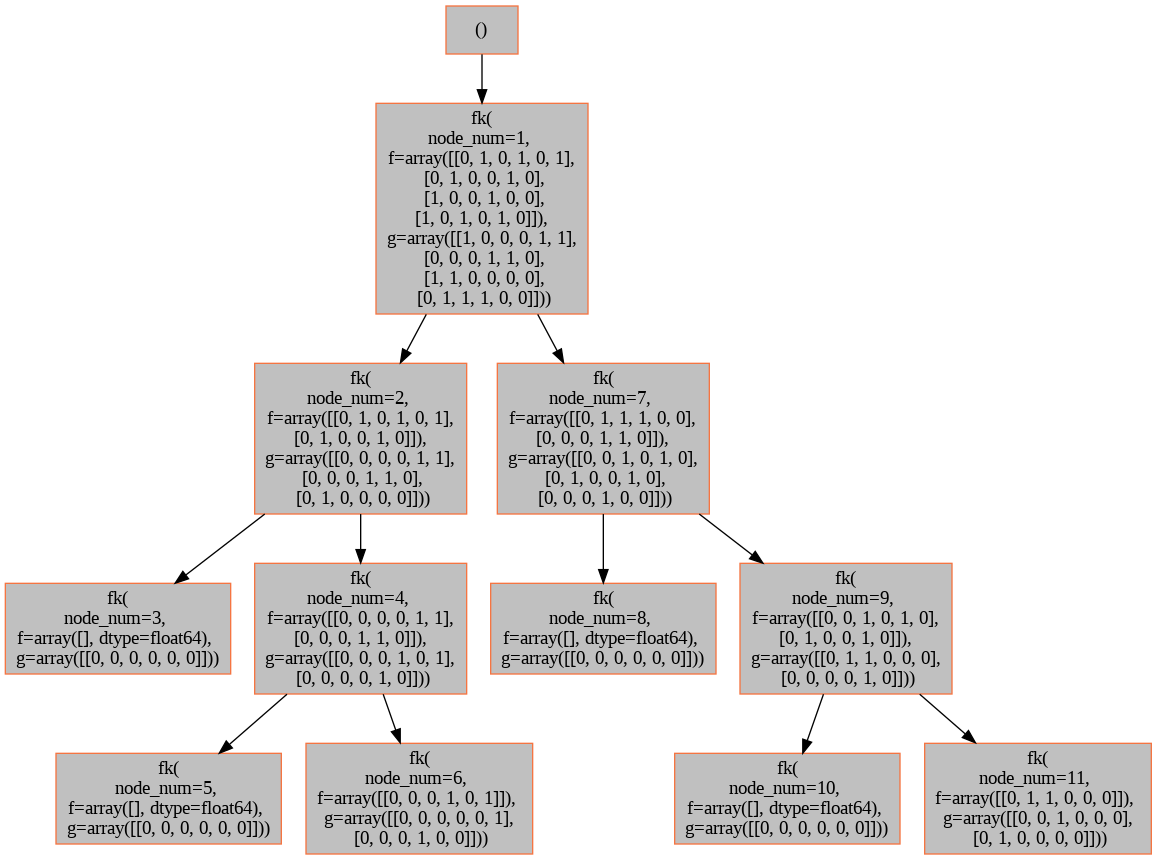
\includegraphics[width=\linewidth]{figures/6a-fka.png}\caption{Visualization of 6-$A$ in \FKA}\end{subfigure}\hfill
\begin{subfigure}{0.48\linewidth}\centering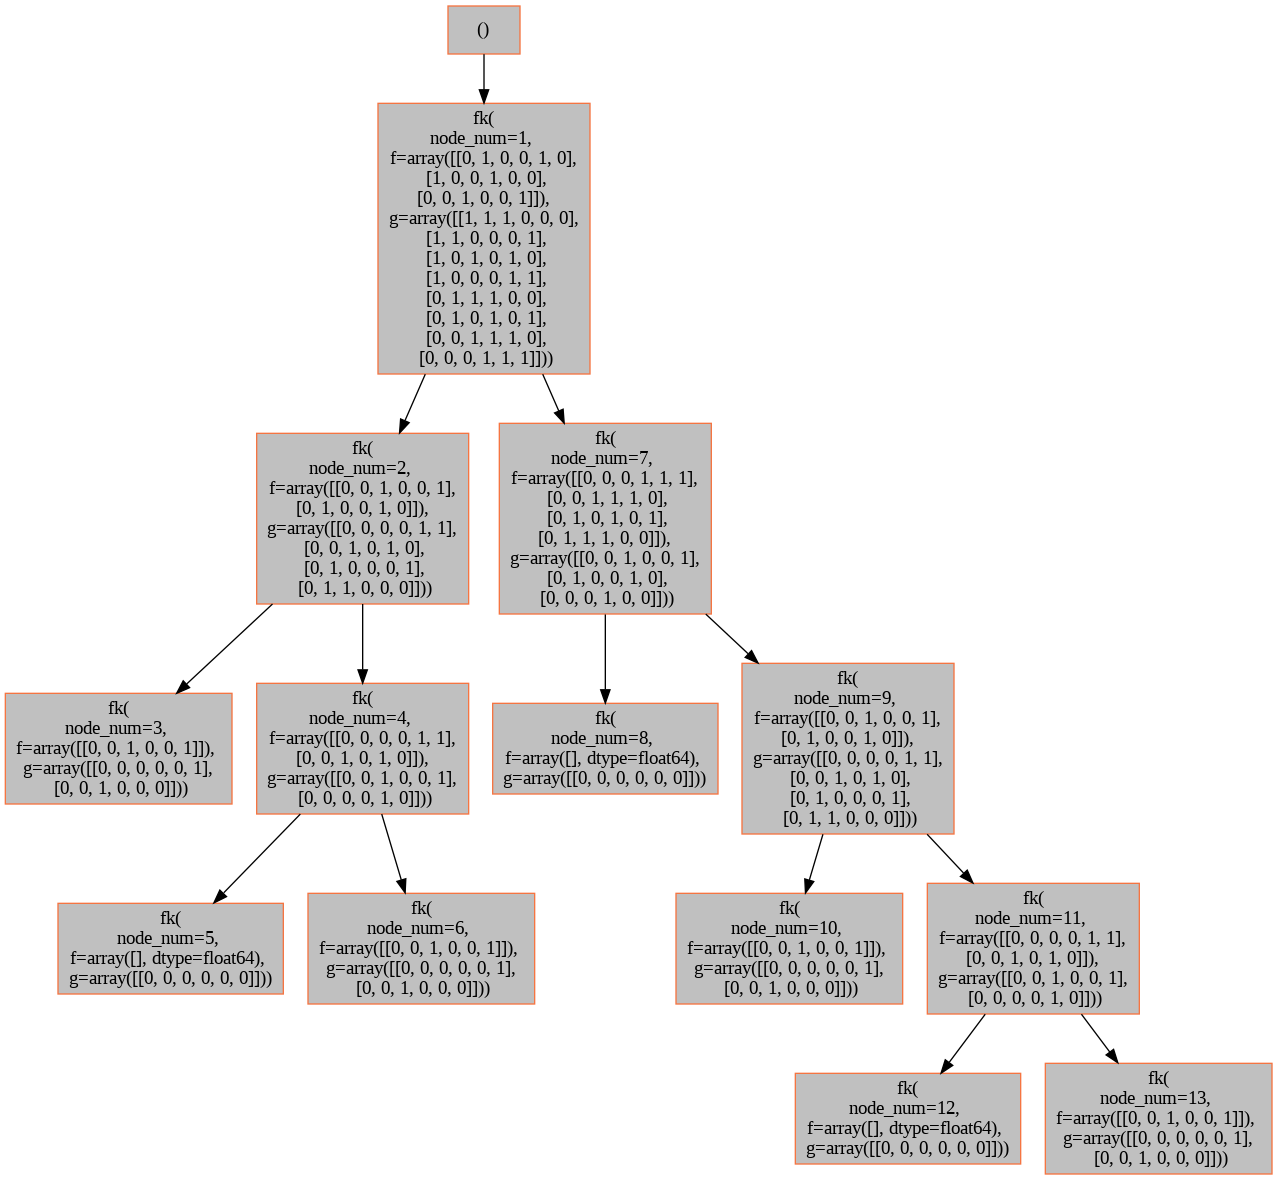
\includegraphics[width=\linewidth]{figures/6b-fka.png}\caption{Visualization of 6-$B$ in \FKA}\end{subfigure}\\[6pt]
\begin{subfigure}{0.48\linewidth}\centering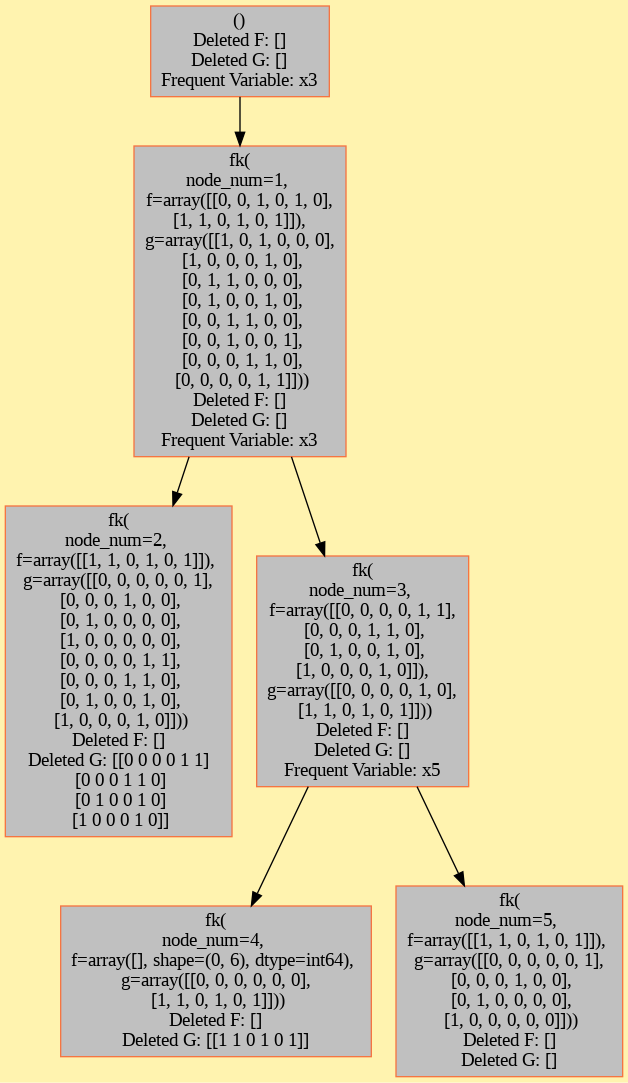
\includegraphics[width=0.85\linewidth]{figures/6c-fka.png}\caption{Visualization of 6-$C$ in \FKA}\end{subfigure}\hfill
\begin{subfigure}{0.48\linewidth}\centering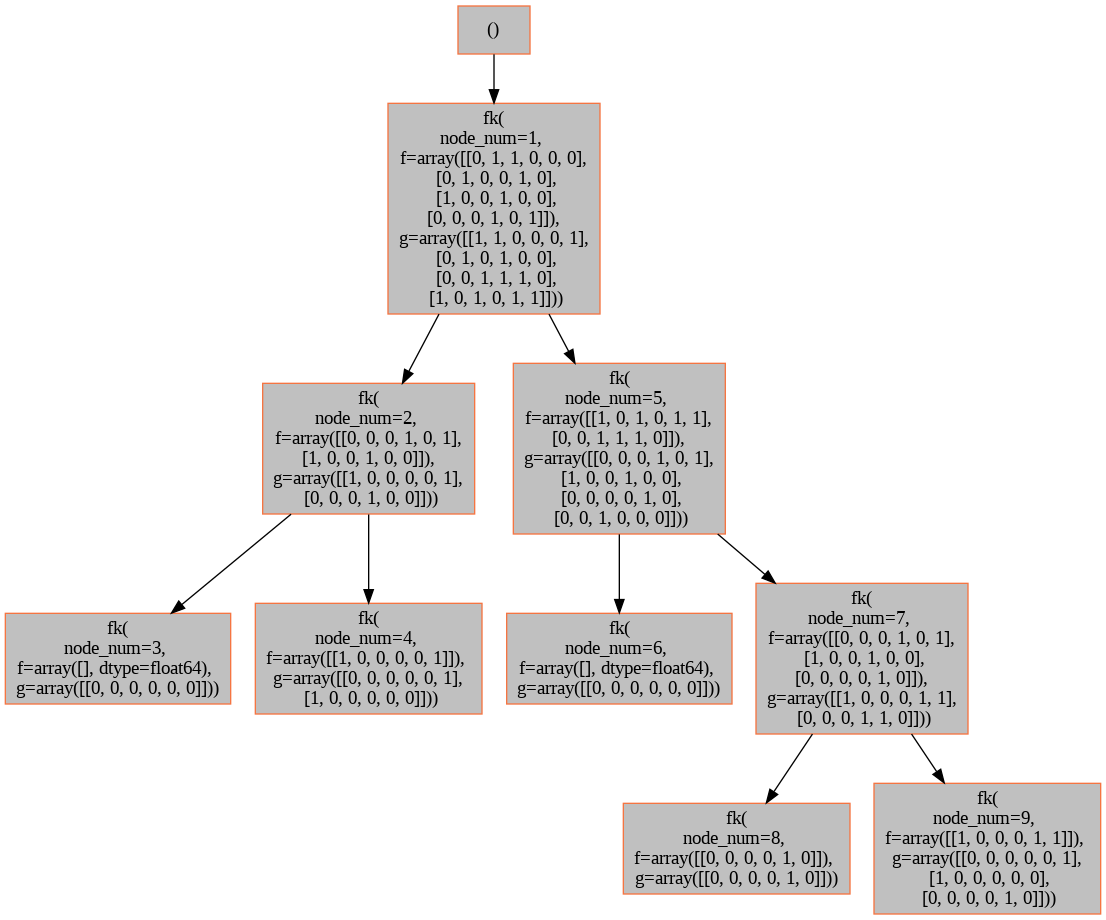
\includegraphics[width=\linewidth]{figures/6d-fka.png}\caption{Visualization of 6-$D$ in \FKA}\end{subfigure}
\caption{Visualizations of hypergraphs on 6 vertices in \FKA}
\end{figure}

\begin{figure}[p]
\centering
\begin{subfigure}{0.48\linewidth}\centering\resizebox{\linewidth}{!}{\begin{forest}
autotree
[{\anode{1}{$v_{1}$}{$C_2\times C_2$}{Conformal}{Perfect}}
  [{\anode{2}{$v_{2}$}{$C_2$}{$\alpha$-acyclic, ROH}{}}
    [{\anode{3}{}{$\{\}$}{}{}}]
    [{\anode{4}{$v_{5}$}{$C_2$}{$\alpha$-acyclic, ROH}{}}
      [{\anode{5}{}{$\{\}$}{}{}}]
      [{\anode{6}{}{$C_2$}{}{}}]
    ]
  ]
  [{\anode{7}{$v_{4}$}{$C_2$}{$\alpha$-acyclic, ROH}{}}
    [{\anode{8}{}{$\{\}$}{}{}}]
    [{\anode{9}{$v_{5}$}{$C_2$}{$\alpha$-acyclic, ROH}{}}
      [{\anode{10}{}{$\{\}$}{}{}}]
      [{\anode{11}{}{$C_2$}{}{}}]
    ]
  ]
]
\end{forest}
}\caption{Automorphism Tree of Hypergraph $6A$ from \cite{SS24} in \FKA.}\end{subfigure}\hfill
\begin{subfigure}{0.48\linewidth}\centering\resizebox{\linewidth}{!}{\begin{forest}
autotree
[{\anode{1}{$v_{1}$}{$C_2\times S_4$}{$\alpha$-acyclic, ROH}{Bipartite}}
  [{\anode{2}{$v_{2}$}{$D_4$}{}{$C_4$ graph}}
    [{\anode{3}{}{$C_2$}{}{}}]
    [{\anode{4}{$v_{5}$}{$C_2$}{}{}}
      [{\anode{5}{}{$\{\}$}{}{}}]
      [{\anode{6}{}{$C_2$}{}{}}]
    ]
  ]
  [{\anode{7}{$v_{4}$}{$D_4$}{ROH}{}}
    [{\anode{8}{}{$\{\}$}{}{}}]
    [{\anode{9}{$v_{2}$}{$D_4$}{}{$C_4$ graph}}
      [{\anode{10}{}{$C_2$}{}{}}]
      [{\anode{11}{$v_{5}$}{$C_2$}{}{}}
        [{\anode{12}{}{$\{\}$}{}{}}]
        [{\anode{13}{}{$C_2$}{}{}}]
      ]
    ]
  ]
]
\end{forest}
}\caption{Automorphism Tree of ROH Hypergraph $6B$ from \cite{SS24} in \FKA.}\end{subfigure}\\[10pt]
\begin{subfigure}{0.48\linewidth}\centering\resizebox{0.8\linewidth}{!}{\begin{forest}
autotree, for tree={font=\small}
[{\anode{1}{$v_{3}$}{$C_2\times S_4$}{ROH, $\alpha$-acyclic}{}}
  [{\anode{2}{}{$S_4$}{}{}}]
  [{\anode{3}{$v_{5}$}{$S_4$}{ROH, $\alpha$-acyclic}{Bipartite}}
    [{\anode{4}{}{$\{\}$}{}{}}]
    [{\anode{5}{}{$S_4$}{}{}}]
  ]
]
\end{forest}
}\caption{Automorphism Tree of ROH Hypergraph $6C$ from \cite{SS24} in \FKA.}\end{subfigure}\hfill
\begin{subfigure}{0.48\linewidth}\centering\resizebox{\linewidth}{!}{\begin{forest}
autotree
[{\anode{1}{$v_{2}$}{$D_4$}{ROH, $\alpha$-acyclic}{Bipartite}}
  [{\anode{2}{$v_{4}$}{$C_2$}{}{}}
    [{\anode{3}{}{$\{\}$}{}{}}]
    [{\anode{4}{}{$C_2$}{}{}}]
  ]
  [{\anode{5}{$v_{3}$}{$C_2\times C_2$}{ROH, $\alpha$-acyclic}{}}
    [{\anode{6}{}{$\{\}$}{}{}}]
    [{\anode{7}{$v_{4}$}{$C_2$}{}{}}
      [{\anode{8}{}{$C_1$}{}{}}]
      [{\anode{9}{}{$S_3$}{}{}}]
    ]
  ]
]
\end{forest}
}\caption{Automorphism Tree of Hypergraph $6D$ from \cite{SS24} in \FKA.}\end{subfigure}
\caption{\FKA{} recursion tree and automorphism tree of $6A$, $6B$, $6C$, and $6D$}
\end{figure}

\section{Future Direction}

Future research can examine the connections between hypergraph coloring, symmetry, and the \FKA{} recursion. Hypergraph $k$-coloring partitions a vertex set into $k$ sets, inducing symmetry within the coloring. However, it is unclear how \FKA{} performs when these colored hypergraphs are used as input. Investigating this relationship could provide new insights into both hypergraph coloring and the behavior of \FKA{} under symmetric constraints.

Another direction involves studying the behavior of \FKA{} on various types of acyclic hypergraphs. While $\alpha$-acyclic hypergraphs are well-studied, other forms of acyclic hypergraphs might influence the algorithm differently. Analyzing their primal graphs and how specific properties are preserved during recursion may uncover new classes of hypergraphs where \FKA{} is less efficient. Additionally, identifying hypergraphs and their transversals that cause \FKA{} to perform poorly can help expanding the upper bounds on \FKA. Recent decomposition methods have used twin vertices to simplify graphs and hypergraphs, and have proven effective in creating efficient algorithms \cite{RMN06}. Applying such techniques to \FKA{} is another avenue of research to pursue.
